\section{Das offene arithmetische Periodensystem}
\label{sec:offenes_periodensystem}

\subsection{Motivation}

Die natürlichen Zahlen werden in der klassischen Zahlentheorie gewöhnlich als linear geordnete Folge betrachtet. 
Im vorliegenden Zugang schlagen wir stattdessen vor, sie als Zustände eines \emph{offenen arithmetischen Periodensystems} zu lesen. 
Der Ausdruck ``Periodensystem'' ist dabei nicht im Sinn einer endlichen, abgeschlossenen Tabelle zu verstehen, sondern als Bezeichnung für eine schalenartige, gruppierte und nach oben offene Ordnungsstruktur.

Die leitende Idee lautet:
\begin{quote}
	Jede natürliche Zahl \(N\) trägt eine mehrschichtige arithmetische Signatur, die sich aus Basisschalen, Restgeneratoren, internen Klassen und modulierenden Strukturgrößen zusammensetzt.
\end{quote}

Im Unterschied zum chemischen Periodensystem ist dieses Schema nicht endlich. 
Es wächst mit jedem neu auftretenden Primträger weiter und bleibt daher \emph{offen nach oben}.

\subsection{Basisschalen}

Für jede natürliche Zahl \(N\in\mathbb{N}\) betrachten wir die p-adischen Bewertungen bezüglich der drei Basen \(2,3,5\):
\[
\nu_2(N),\qquad \nu_3(N),\qquad \nu_5(N).
\]
Diese Größen geben an, wie tief \(N\) in den dyadischen, triadischen und pentadischen Basisschalen sitzt.

Die Basisschalenwelt wird erzeugt durch die Familien
\[
2^n,\qquad 3^m,\qquad 2^n3^m,\qquad 2^n3^m5^o,
\]
wobei \(n,m,o\ge 0\) ganze Zahlen sind.
Damit besitzt jede Zahl zunächst eine Position in einem logarithmisch organisierten Schalenraum.

\begin{definition}[2-3-5-Rest]
	Für \(N\in\mathbb{N}\) definieren wir den \emph{2-3-5-Rest}
	\[
	R_{235}(N):=\frac{N}{2^{\nu_2(N)}3^{\nu_3(N)}5^{\nu_5(N)}}.
	\]
\end{definition}

Dieser Rest misst, ob \(N\) vollständig in der Basisschalenwelt liegt oder ob zusätzliche Generatorstruktur vorhanden ist:
\[
R_{235}(N)=1
\quad\Longleftrightarrow\quad
N \text{ liegt vollständig in der 2-3-5-Welt.}
\]

\subsection{Interne Vierergruppenstruktur}

Nach Herausziehen aller Faktoren \(2\) und \(3\) betrachten wir die reduzierte Restklasse modulo \(12\). 
Dadurch erhalten wir die vier Klassen
\[
e,\quad a,\quad b,\quad c,
\]
mit der Identifikation
\[
1\mapsto e,\qquad 5\mapsto a,\qquad 7\mapsto b,\qquad 11\mapsto c.
\]
Diese vier Klassen bilden die Kleinsche Vierergruppe
\[
V_4=\{e,a,b,c\}.
\]

\begin{definition}[EABC-Klasse]
	Die \emph{EABC-Klasse} einer Zahl \(N\) ist die Klasse
	\[
	u(N)\in\{e,a,b,c\},
	\]
	die aus der modulo-\(12\)-Reduktion des nach \(2\)- und \(3\)-Faktoren bereinigten Restes gewonnen wird.
\end{definition}

Die EABC-Klassen spielen im offenen arithmetischen Periodensystem die Rolle interner Familien.

\subsection{Vier Modifikationsmodule}

Zur Basisschalen- und Reststruktur treten vier modulierende Operatoren hinzu.

\paragraph{(i) von Klitzing-Modul.}
Das von-Klitzing-Modul modelliert robuste Stufen- bzw.\ Plateau-Bildung. 
Es beschreibt die Tendenz, dass arithmetische Zustände nicht beliebig fein variieren, sondern sich auf diskrete Niveaus organisieren.

\paragraph{(ii) Aharonov--Bohm-Modul.}
Das Aharonov--Bohm-Modul liefert eine arithmetische Phase und beschreibt, dass Zahlen nicht nur lokal durch Faktorisierung, sondern auch durch zyklische Umlaufstruktur charakterisiert werden können.

\paragraph{(iii) Morley--Walter-Modul.}
Das Morley--Walter-Modul erfasst geometrische Kopplung zwischen den Schalenexponenten, insbesondere dann, wenn mehrere Basisschalen gleichzeitig aktiv sind.

\paragraph{(iv) Kepler-Modul.}
Das Kepler-Modul misst die Harmonie bzw.\ Einbettung einer Zahl in die globale Schalenordnung. 
Es bewertet, wie stark \(N\) in die Basisschalenwelt integriert ist.

\subsection{Erste diskrete Realisierung der Strukturgrößen}

Für eine erste diskrete Modellierung setzen wir die folgenden Hilfsgrößen an.

\begin{definition}[AB-Index]
	Der \emph{arithmetische Phasenindex} sei gegeben durch
	\[
	\phi_{\mathrm{AB}}^{(0)}(N)
	=
	\nu_2(N)+2\nu_3(N)+3\nu_5(N)+\chi_4(u(N)),
	\]
	wobei
	\[
	\chi_4(e)=0,\qquad
	\chi_4(a)=1,\qquad
	\chi_4(b)=2,\qquad
	\chi_4(c)=3.
	\]
\end{definition}

\begin{definition}[Morley--Walter-Kopplung]
	Wir definieren die erste diskrete Morley--Walter-Kopplung durch
	\[
	M_{\mathrm{MW}}(N)
	=
	\nu_2(N)\nu_3(N)+\nu_3(N)\nu_5(N)+\nu_2(N)\nu_5(N).
	\]
\end{definition}

Diese Größe ist genau dann positiv, wenn mehrere Basisschalen gleichzeitig aktiv sind.

\begin{definition}[Kepler-Harmonie]
	Die erste Kepler-Harmoniezahl sei
	\[
	K_{\mathrm{Kep}}(N)
	=
	\nu_2(N)+\nu_3(N)+\nu_5(N).
	\]
\end{definition}

\begin{definition}[von-Klitzing-Plateau]
	Als einfache diskrete Plateaugröße setzen wir
	\[
	Q_{\mathrm{vK}}(N)
	=
	M_{\mathrm{MW}}(N)+K_{\mathrm{Kep}}(N).
	\]
\end{definition}

\subsection{Zustandsvektor}

Damit erhält jede Zahl \(N\) einen strukturierten arithmetischen Zustandsvektor
\[
\mathcal P(N)
=
\bigl(
\nu_2(N),\nu_3(N),\nu_5(N),
R_{235}(N),
u(N),
\phi_{\mathrm{AB}}^{(0)}(N),
M_{\mathrm{MW}}(N),
K_{\mathrm{Kep}}(N),
Q_{\mathrm{vK}}(N)
\bigr).
\]

\begin{definition}[Offenes arithmetisches Periodensystem]
	Das \emph{offene arithmetische Periodensystem} ist die Klassifikation der natürlichen Zahlen \(N\in\mathbb{N}\) durch den Zustandsvektor
	\[
	\mathcal P(N)
	=
	(\text{Schale},\text{Restgenerator},\text{Gruppe},\text{Phase},\text{Geometrie},\text{Harmonie},\text{Plateau}).
	\]
\end{definition}

\subsection{Statusklassen}

Um das System nicht nur numerisch, sondern auch phänomenologisch lesbar zu machen, führen wir Statusklassen ein.

\begin{definition}[Status]
	Jeder Zahl \(N\) wird ein Status
	\[
	\Sigma(N)\in
	\{
	\text{Basis},
	\text{a-Schale},
	\text{Misch-Basis},
	\text{Plateau},
	\text{Plateauwechsel},
	\text{neuer Generator},
	\text{harmonischer Nachläufer},
	\text{Mischzahl}
	\}
	\]
	zugeordnet.
\end{definition}

Die Interpretation ist wie folgt:
\begin{itemize}
	\item \textbf{Basis}: \(R_{235}(N)=1\), keine zusätzliche Restgeneratorstruktur.
	\item \textbf{a-Schale}: pentadisch betonte Basisschicht.
	\item \textbf{Misch-Basis}: mehrere Basisschalen zugleich aktiv.
	\item \textbf{Plateau / Plateauwechsel}: robuste Stufenstruktur der Zahl.
	\item \textbf{neuer Generator}: \(R_{235}(N)\) ist ein neuer Primträger \(>5\).
	\item \textbf{harmonischer Nachläufer}: \(N\) ist Vielfaches oder Fortsetzung eines bereits eingeführten Generators.
	\item \textbf{Mischzahl}: hybride Rest- und Schalenstruktur.
\end{itemize}

\subsection{Gruppen und Perioden}

Im offenen arithmetischen Periodensystem sind Gruppen und Perioden im Allgemeinen nicht endlich.

\begin{itemize}
	\item \textbf{Gruppen} sind Familien gleicher interner Struktur, etwa gleiche EABC-Klasse oder gleicher Restgenerator.
	\item \textbf{Perioden} sind offene Schalenabschnitte, in denen dieselbe Basisschalenarchitektur dominiert, bevor neue Generatoren die Ordnung erweitern.
\end{itemize}

Dadurch ist das System zwar periodisch im strukturellen Sinn, aber offen im arithmetischen Sinn.

\subsection{Mendelejew-Analogie}

Die Analogie zu einem Periodensystem im Sinn Mendelejews ist nicht bloß metaphorisch. 
Das System
\begin{enumerate}
	\item ordnet bekannte arithmetische Zustände,
	\item trennt Familien und Perioden,
	\item markiert Übergänge und Lücken,
	\item und lässt offene Fortsetzungen durch neue Generatoren zu.
\end{enumerate}

Es handelt sich daher nicht bloß um eine alternative Schreibweise der Faktorisierung, sondern um ein Klassifikationsschema mit gruppierter, schalenartiger und generatoroffener Struktur.

\subsection{Erste empirische Tafel}

Für \(N\le 300\) ergibt sich bereits eine verfeinerte Tafel, in der die offenen Generatoren in vertikale Familien nach EABC-Klasse zerfallen. 
Insbesondere erscheinen bereits Familien der Form
\[
e:\mathrm{Gen},\qquad a:\mathrm{Gen},\qquad b:\mathrm{Gen},\qquad c:\mathrm{Gen},
\]
während Plateaus, Nachläufer und Mischzahlen als eigene Sekundärzustände sichtbar werden.

\begin{figure}[t]
	\centering
	% Datei anpassen oder in dein figures/-Verzeichnis legen
	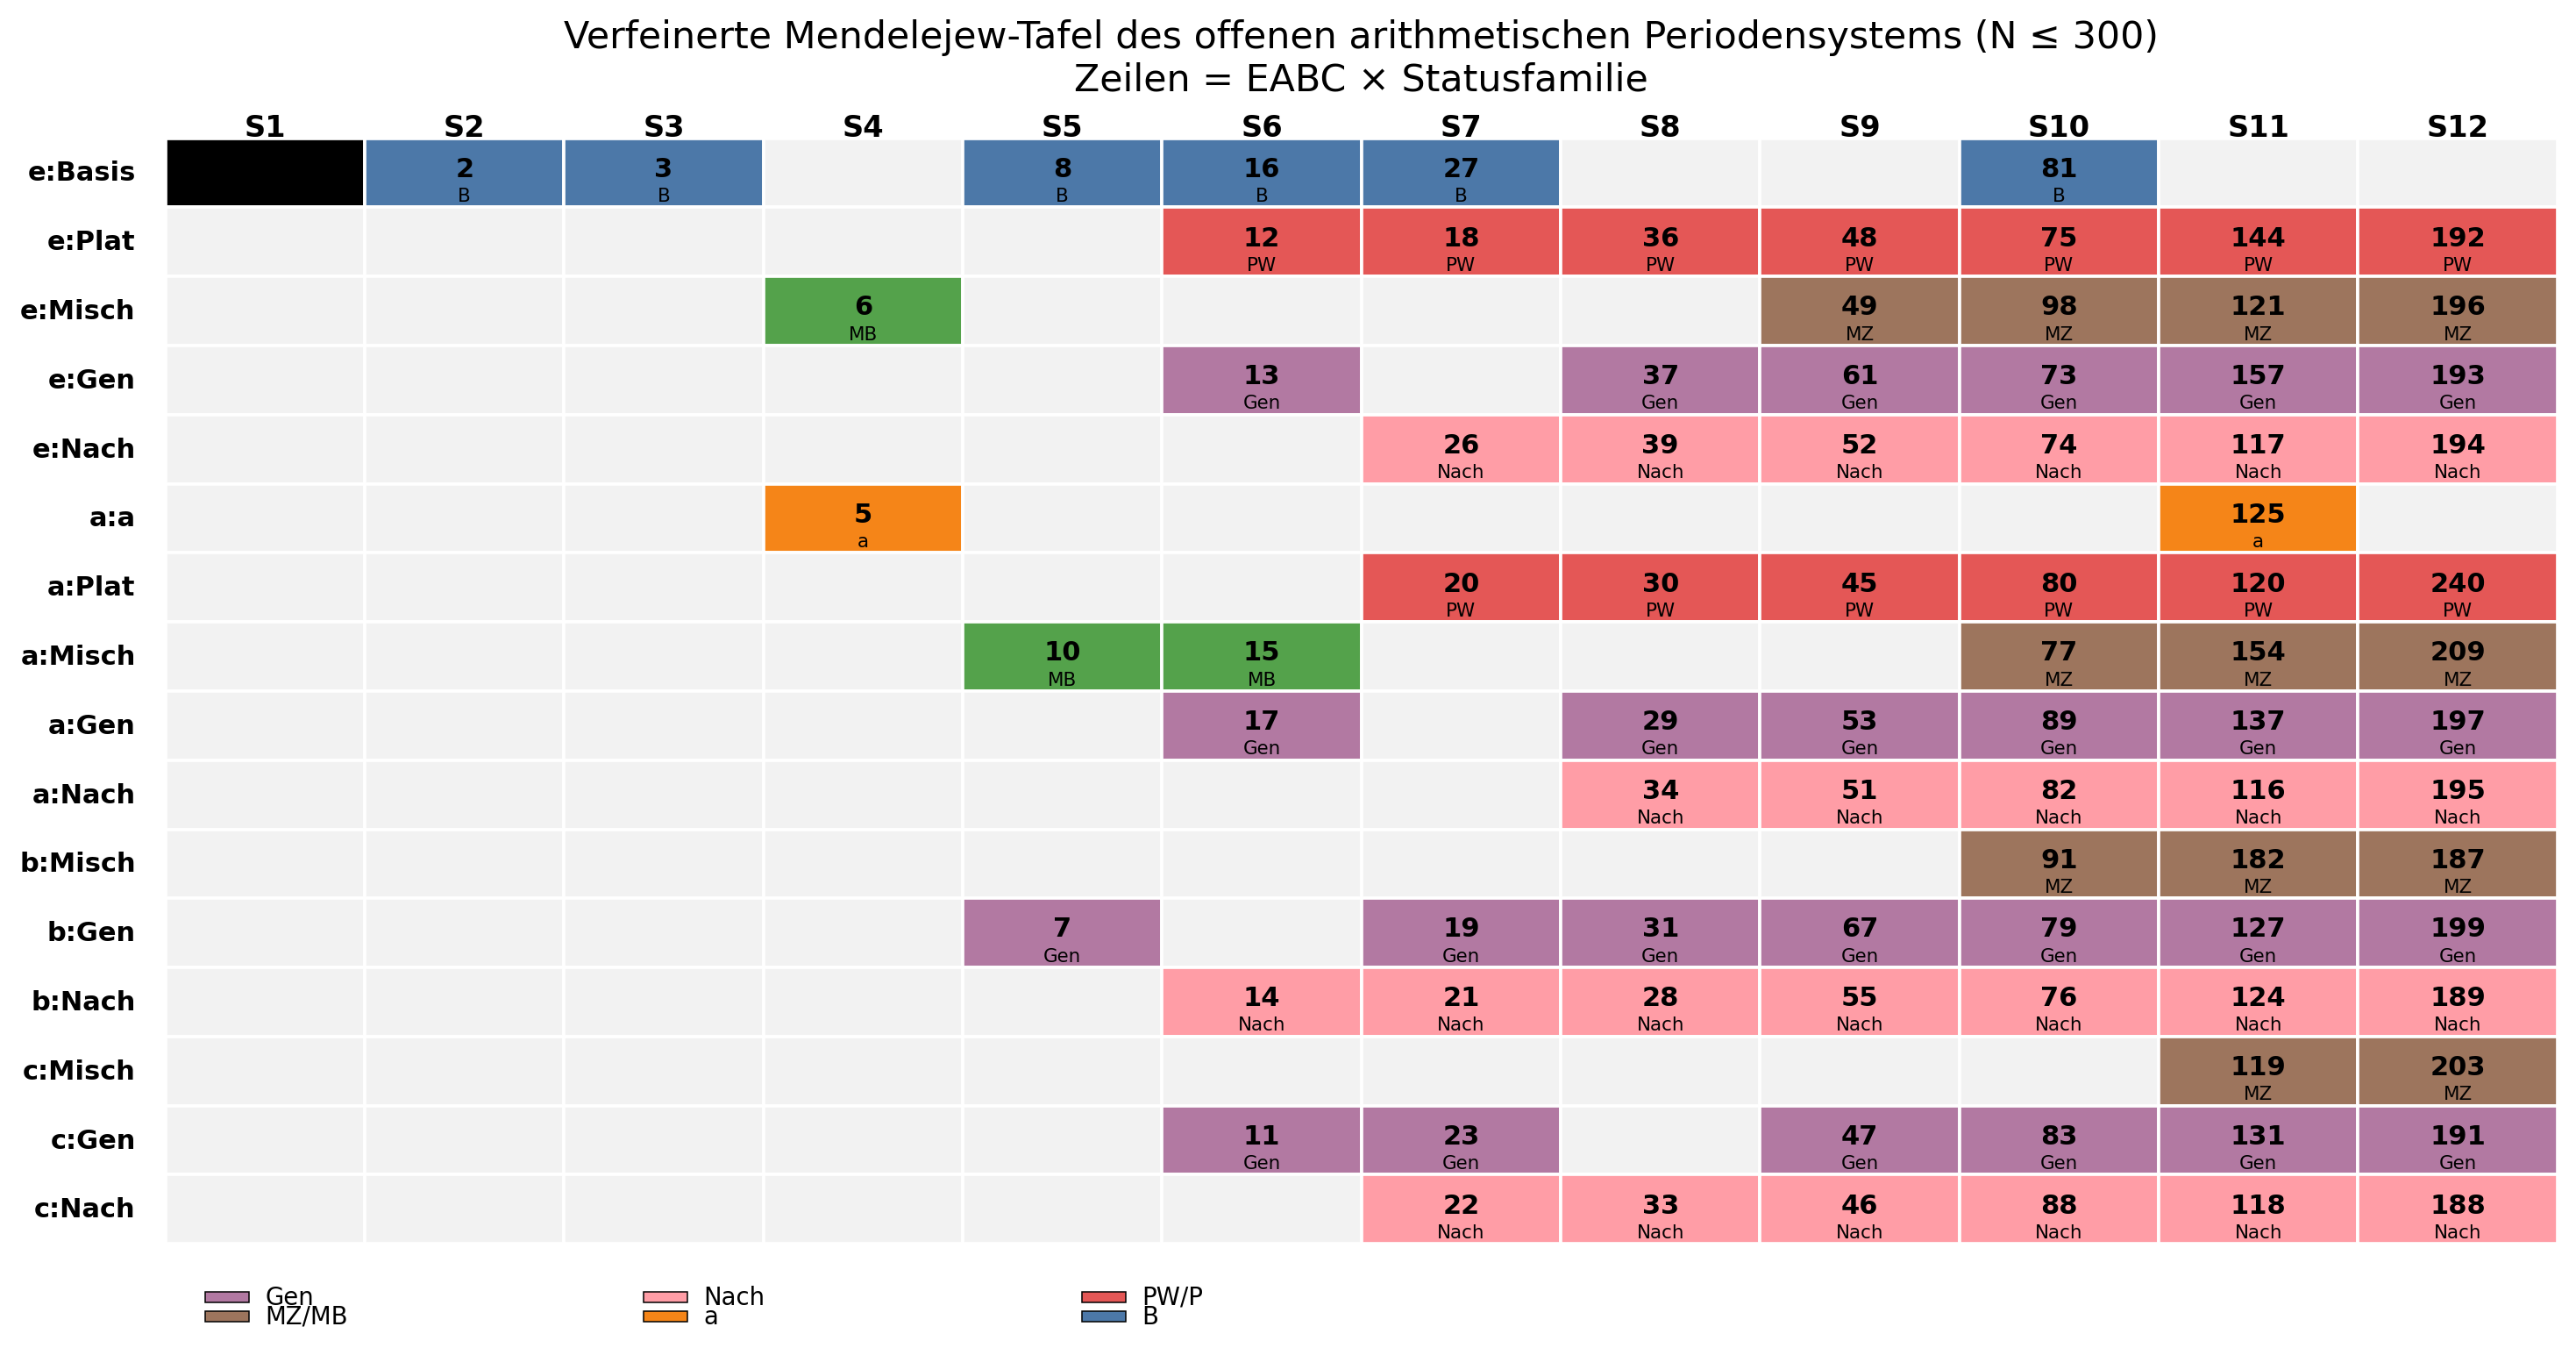
\includegraphics[width=\textwidth]{offenes_arithmetisches_mendelejew_tafel_bis_300_verfeinert.png}
	\caption{Verfeinerte Mendelejew-Tafel des offenen arithmetischen Periodensystems für \(N\le 300\). Die Spalten kodieren verdichtete Schalenbereiche, die Zeilen EABC-Klasse und Statusfamilie.}
	\label{fig:open_arithmetic_periodic_table}
\end{figure}

\subsection{Ausblick}

Die vorliegende Fassung ist als erste diskrete Rohform zu verstehen. 
Die nächsten Schritte bestehen darin,
\begin{itemize}
	\item die Tafel auf größere Bereiche \(N\le 1000\) oder \(N\le 5000\) auszuweiten,
	\item Triggerfunktionen wie \(\Theta(N)\) oder \(\Pi_{\mathrm{open}}(N)\) direkt einzubinden,
	\item die Familienbildung mit generatorischen und phasenartigen Selektionsregeln zu koppeln,
	\item sowie die Struktur mit BM-Datenquellen, AHPN-Listen oder weiteren Normklassen abzugleichen.
\end{itemize}

Damit könnte aus der hier vorgeschlagenen Rohform ein systematisches arithmetisches Ordnungsmodell entstehen.